\section{A finite planar distribution protocol}
\label{sec:geometry}

We now construct a schedule to which the compression rule applies.
The parties will be attached to dyadic squares.  Their memories need not
be spatially localized: a party may initially hold an entire auxiliary
copy of $\Omega$, and may act on all of its own registers.  What we must
control is the number of parties involved in a gate, each party's total
participation in gates with other parties, and the distances between the
squares to which those parties are attached.

\begin{proposition}[Distribution through a dyadic hierarchy]
\label{prop:protocol}
For all sufficiently large $L$, there is a protocol with the following
properties.  All constants in this statement are uniform in the
Hamiltonian and $L$.
\begin{enumerate}
\item
There are $O(L^2)$ parties, one for each square in a padded dyadic
hierarchy and at most a fixed number of additional parties for each
repainting of a square.  Initialization is a pure product across
parties.  One party initially holds the main copy of $\Omega$; all
auxiliary copies are initialized privately at their designated parties.
\item
The schedule has at most $C L^3$ changes.  Each change is implemented by
a fixed number of contraction gates involving at most a fixed number of
parties and having the bipartite-resource expansions established in
Lemmas~\ref{lem:small-rewrite}, \ref{lem:birth}, and
\ref{lem:exchange}.  The expansions can be made accurate to any fixed
inverse power of $L$ in operator norm where an approximation is needed.
Each party participates in at most a fixed number of gates involving
other parties over its entire lifetime.
\item
Every linked gate involves parties at the same or adjacent dyadic
scales.  Parties at a gate have addresses at distance $O(n)$ from one
another, where $n$ is either endpoint scale; additional parties have the
scale and address of the square to whose repainting they belong.
\item
There is a designated reference vector at every stage, formed from the
main encoded frame and the auxiliary encoded frames.  All its factors
have norm at most one.  Each change takes its preceding reference vector
within $C L^{-20}$ in vector norm of its following reference vector.
At the end, the reference is
\[
 \Omega\otimes\Xi,
 \qquad 1-C L^{3-60}\le \norm{\Xi}\le1,
\]
where $\Xi$ contains only registers to be discarded.  Every original
physical site is a raw register at its own unit-square party.  No other
party has a physical output, so every party's physical output dimension
is at most $q$.
\end{enumerate}
\end{proposition}

The conservative exponent $3$ in the schedule and reference-norm bounds
will be convenient for error accounting.  The construction below in fact
has $O(L^2)$ changes.  We prove the proposition by specifying all its
guides and verifying the hypotheses of the three frame operations.

\subsection{Ambient guides, holes, and the hierarchy}

Translate the lattice so that its sites are the cell centers
$(i+\tfrac12,j+\tfrac12)$, $0\le i,j<L$.  Let $N$ be a power of two
with $L\le N<2L$.  The dyadic hierarchy consists of the aligned squares
in $[0,N]^2$ of side $n=2^j$, including the root square.  Unoccupied
cells of this padded square carry no registers.  A different party is
assigned to each dyadic square.

A \emph{guide} is a finite polygonal partition of the ambient plane,
whose labels name the parties owning the raw registers at its sampled
sites.  All guides below are specified by their open polygonal chambers.
Use one consistent tie convention for all boundaries in the finite
schedule: move a sampled point by an arbitrarily small generic vector
into an incident chamber, consistently across all descriptions, and
take the resulting label.  Equivalently, choose a sufficiently small
generic displacement after all the finitely many guides are specified.
No label is introduced solely on a boundary face.  Separation estimates
will be stated for closures, and consequently remain valid for these
sampled labels.  Squares used for the patch constraints retain their
closed-square sampling convention.

We pass successively from the uniform assignment by $2n$-squares to the
uniform assignment by $n$-squares, for
$n=N/2,N/4,\ldots,1$.  At a given level, view each old $2n$-square
label as constant on its four $n$-square children, and repaint one
$n$-square at a time to its new party.  At the beginning and end of a
repainting, every other $n$-square has either its old $2n$-square label
or its final $n$-square label.  In particular, the guide along an open
edge of the square being repainted has a single label on each side.

At the beginning and end of such a repainting, the exterior of
$[0,N]^2$ has one placeholder label.  During that repainting it is
represented by a fresh additional party attached to the square being
repainted.  At the next repainting its identity may be replaced.  This
does not transfer any main raw register: at those transition times the
placeholder owns no physical main-sheet site.  We will also ensure that
it holds no persistent main-sheet tag.  Temporary operations may give
it physical main-sheet registers within a treated neighborhood, but the
repainting restores the prescribed exterior assignment before that party
is retired.

Fix, in an order made precise below, constants $D>0$ and
$\epsilon_0>0$, and write
\begin{equation}
 t=D\log L,
 \qquad h_n=\epsilon_0\min(n,t).
 \label{eq:geometry-scales}
\end{equation}
A \emph{true vertex} of a guide is a point lying in the closures of at
least three distinct actual labels.  The guides we construct have only
finitely many such points.  At every true vertex use the encoded hole
of Definition~\ref{def:frame}, with inner radius $h_n$ and outer radius
$2h_n$, and with test exponent $60$.  We will choose $\epsilon_0$ so
that the outer squares are disjoint within each guide.  For a given
center and radius, make the same choice of the adaptive constraint on
every sheet.  Thus each branch of a hole uses a square with radius
between $h_n$ and $2h_n$.

Choose the tag holder canonically among the actual incident labels
other than the placeholder, for example by a fixed order on genuine
block parties.  The placeholder is omitted from this choice, regardless
of its current identity.  A true vertex has at least two other incident
labels, so the rule is always possible.  An empty physical outer square
uses the trivial one-branch encoding.  When a guide is exchanged between
sheets, use the same tag rule; its tag then accompanies the whole hole.

Before entering a new hierarchy level, resize existing main-sheet holes
to its value of $h_n$, one hole at a time, without changing the guide.
These resizings will also be small-patch rewrites.  A fresh auxiliary
sheet has a uniform guide on the whole plane and therefore no holes.
An auxiliary sheet that has been retired is kept idle, with its
registers and tags at their current parties, until the final discard.
Its holes are not resized at subsequent levels.

\subsection{The edge construction before point treatment}

Choose a large fixed constant $K_0$.  For $n\le K_0t$ we will repaint
the square directly by a small-patch rewrite.  We first describe the
large-scale construction, for $n>K_0t$, before treating its finitely
many contact points.

Let $S$ be the $n$-square being repainted, with old label $A$ and final
label $B$.  For any of its edges let $s\in(0,n)$ be the coordinate
parallel to that edge, measured from one endpoint, and let $d$ be the
normal coordinate, positive into $S$.  Set
\begin{equation}
 w(s)=10^{-3}\min(s,n-s),
 \qquad x=\frac{d}{w(s)}.
 \label{eq:geometry-band}
\end{equation}
An interval in $x$ always refers only to this parallel-coordinate span.
These intervals define polygonal bands, with their only bends at
$s=n/2$.

First birth $B$ in the central part of $S$, leaving the four inward
edge bands $0<x<1$ with label $A$.  More explicitly, the changed open
chambers are the points of the interior of $S$ lying beyond the
$x=1$ boundary for every edge.  Their closure meets the exterior of
$S$ only at the four corners.  These four corners are the marked
contact points for this birth.  Now process the four edges one at a
time.  At the start of an edge operation its normal word is
\[
 C\quad A\quad B,
 \qquad x<0,\quad 0<x<1,\quad x>1,
\]
in the neighborhood of the edge.  Here $C$ is the label on the unique
exterior neighboring $n$-square, or the placeholder at an exterior
edge.  Nominal names in all the words below are permitted to coincide;
adjacent equal labels are simply one actual region.  The marked points
for an edge operation are its two endpoints.

The reason for using an auxiliary sheet is already visible when $A,B,C$
are distinct.  A direct death of the $A$ strip into $B$ would leave the
surrounding word $C\mid B$.  The closure of the changed strip meets $C$
along the entire original edge, so it has zero separation from the
non-$B$ owners.  The angular-information estimate therefore does not
supply the hypothesis needed for Lemma~\ref{lem:birth}.  We instead prepare
additional $A$ and $B$ strips on an auxiliary sheet and exchange them into
the exterior.  The resulting $C$ strip is surrounded by $A$ and can die
into it; the combined $A$ strip is then surrounded by $B$ and can die in
turn.  A final birth and death restore the original exterior assignment.
The construction below supplies these buffers away from the endpoints;
the subsequent point treatment supplies the logarithmic clearance there.

Perform the following finite sequence.
\begin{enumerate}
\item
Initialize a fresh auxiliary $\Omega$ sheet uniformly at $C$.  On this
sheet birth $B$ in $-6<x<-1$, then $A$ in $-5<x<-2$, then $C$ in
$-4<x<-3$.  Each insertion lies strictly inside its surrounding band.
The resulting auxiliary word is
\begin{equation}
 C\mid B\mid A\mid C\mid A\mid B\mid C,
 \qquad -6,-5,-4,-3,-2,-1
 \label{eq:geometry-aux-word}
\end{equation}
where the numbers list successive interfaces.
\item
Exchange the two sheet assignments on the lens
\begin{equation}
 Y=\{0<s<n:\ -7<x<-7/2\}.
 \label{eq:geometry-lens}
\end{equation}
Both of its open sides lie in common-$C$ corridors: the side $x=-7$
lies in the auxiliary $C$ sector $x<-6$, and the other passes
through the auxiliary $C$ band $(-4,-3)$.  The main sheet was $C$
throughout this exterior strip.  After the exchange its word is
\begin{equation}
 C\mid B\mid A\mid C\mid A\mid B,
 \qquad -6,-5,-4,0,1.
 \label{eq:geometry-main-word}
\end{equation}
The auxiliary sheet is then retired, after completing the point
treatments for this exchange as described below.
\item
On the main sheet, kill the $C$ band $(-4,0)$ into $A$, and then kill
the resulting $A$ band $(-5,1)$ into $B$.  The word is now $C\mid B$
with interface at $-6$.  Birth $C$ in $(-3,0)$ inside $B$, and kill
the remaining $B$ band $(-6,-3)$ into $C$.  The final word is
$C\mid B$ with interface at zero.
\end{enumerate}

Figure~\ref{fig:geometry-bands} records the complete normal-word
sequence at a fixed parallel coordinate.
\begin{figure}[tbp]
\centering
\begingroup
\newcommand{\geometrybandat}[5]{%
  \path[band#4] (#2,{#1-.20}) rectangle (#3,{#1+.20});
  \node[font=\scriptsize] at ({#5},#1) {$#4$};%
}
\newcommand{\geometryband}[4]{%
  \geometrybandat{#1}{#2}{#3}{#4}{(#2+#3)/2}%
}
\newcommand{\geometryrow}[2]{%
  \node[anchor=east,align=right,font=\scriptsize]
    at (-8.20,#1) {#2};%
}
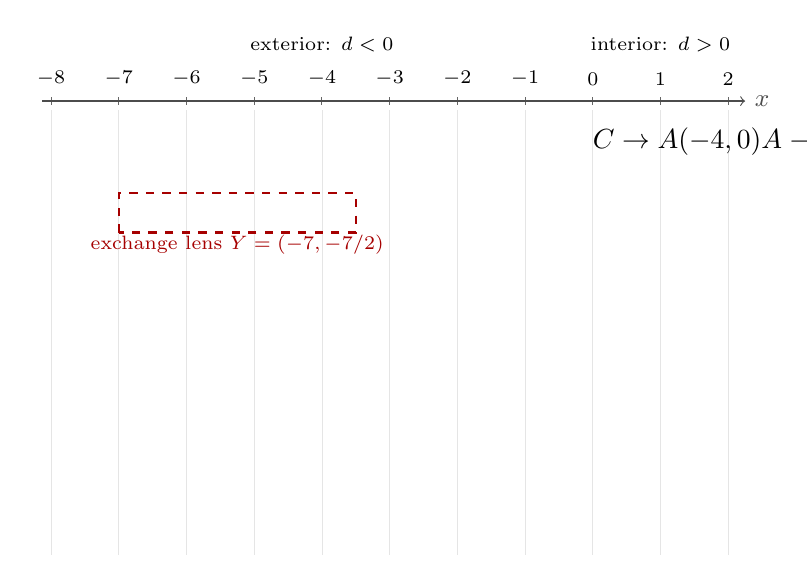
\begin{tikzpicture}[
  x=.86cm,y=1cm,
  bandA/.style={fill=orange!35,draw=black!35,line width=.3pt},
  bandB/.style={fill=cyan!28,draw=black!35,line width=.3pt},
  bandC/.style={fill=black!12,draw=black!35,line width=.3pt},
  lens/.style={draw=red!65!black,dashed,line width=.8pt}
]
  \foreach \geometrytick in {-8,-7,...,2} {
    \draw[black!10,line width=.3pt]
      (\geometrytick,.48) -- (\geometrytick,-5.17);
    \draw[black!60,line width=.35pt]
      (\geometrytick,.55) -- (\geometrytick,.65);
    \node[above,font=\scriptsize] at (\geometrytick,.67)
      {$\geometrytick$};
  }
  \draw[->,black!70] (-8.13,.60) -- (2.25,.60)
    node[right,font=\small] {$x$};
  \node[font=\scriptsize] at (-4,1.32) {exterior: $d<0$};
  \node[font=\scriptsize] at (1,1.32) {interior: $d>0$};

  \geometryrow{0}{\textbf{Main: initial}\\before the exchange}
  \geometryband{0}{-8}{0}{C}
  \geometryband{0}{0}{1}{A}
  \geometryband{0}{1}{2}{B}

  \geometryrow{-.82}{\textbf{Auxiliary}\\three nested births}
  \geometrybandat{-.82}{-8}{-6}{C}{-7.22}
  \geometryband{-.82}{-6}{-5}{B}
  \geometryband{-.82}{-5}{-4}{A}
  \geometrybandat{-.82}{-4}{-3}{C}{-3.72}
  \geometryband{-.82}{-3}{-2}{A}
  \geometryband{-.82}{-2}{-1}{B}
  \geometryband{-.82}{-1}{2}{C}
  \draw[lens] (-7,-1.07) rectangle (-3.5,-.57);
  \node[below,inner sep=0pt,font=\scriptsize,text=red!65!black] at (-5.25,-1.09)
    {exchange lens $Y=(-7,-7/2)$};

  \geometryrow{-1.64}{\textbf{Main: exchange}\\auxiliary retired}
  \geometryband{-1.64}{-8}{-6}{C}
  \geometryband{-1.64}{-6}{-5}{B}
  \geometryband{-1.64}{-5}{-4}{A}
  \geometryband{-1.64}{-4}{0}{C}
  \geometryband{-1.64}{0}{1}{A}
  \geometryband{-1.64}{1}{2}{B}

  \geometryrow{-2.46}{\textbf{Main: first death}\\$C\to A$ on $(-4,0)$}
  \geometryband{-2.46}{-8}{-6}{C}
  \geometryband{-2.46}{-6}{-5}{B}
  \geometryband{-2.46}{-5}{1}{A}
  \geometryband{-2.46}{1}{2}{B}

  \geometryrow{-3.28}{\textbf{Main: second death}\\$A\to B$ on $(-5,1)$}
  \geometryband{-3.28}{-8}{-6}{C}
  \geometryband{-3.28}{-6}{2}{B}

  \geometryrow{-4.10}{\textbf{Main: birth}\\$B\to C$ on $(-3,0)$}
  \geometryband{-4.10}{-8}{-6}{C}
  \geometryband{-4.10}{-6}{-3}{B}
  \geometryband{-4.10}{-3}{0}{C}
  \geometryband{-4.10}{0}{2}{B}

  \geometryrow{-4.92}{\textbf{Main: final death}\\$B\to C$ on $(-6,-3)$}
  \geometryband{-4.92}{-8}{0}{C}
  \geometryband{-4.92}{0}{2}{B}
\end{tikzpicture}
\endgroup
\caption{Normal-band words at one fixed $0<s<n$, in the coordinate
  $x=d/w(s)$ with $w(s)=10^{-3}\min(s,n-s)$; the chart displays only
  $-8\le x\le2$. The auxiliary starts uniformly at $C$ before the three
  nested births shown in its row. Exchanging the two sheets on the dashed
  lens creates the next main row: both displayed transverse boundaries
  lie in $C$ corridors on both sheets. The two deaths leave the interface
  at $x=-6$; the last
  birth and death move it to $x=0$, restoring the exterior label $C$.
  These are nominal labels: $A,B,C$ may coincide. This is a transverse
  schematic away from the edge endpoints and their point treatments.}
\label{fig:geometry-bands}
\end{figure}


Every band used in this sequence is contained in $-8<x<2$.  Such
bands along distinct edges of $S$ have disjoint interiors.  Opposite
edges are separated by $n$, whereas their bands have width at most
$0.004n$ on either relevant side.  For adjacent edges, a common point
in the parallel-coordinate spans would have to lie inside $S$ near
the shared corner.  If its two distances from those edges are $r_1,r_2$,
membership in both enlarged bands would imply
$r_1<0.008r_2$ and $r_2<0.008r_1$, which is impossible.  The negative
part of an edge band lies in its one exterior neighboring square, and
cannot enter the parallel-coordinate span of an adjacent edge.
Consequently an already completed edge does not alter the normal word
needed at the next one.  At the end of the four edge operations $S$
has label $B$ and every other square has its original label.  The same
description is valid along the placeholder exterior: all temporary
plane changes there are restored at the end.

\subsection{Uniform angular separation}

We record precisely the geometry needed to invoke the information
estimate.  For a given elementary operation let $\mathcal V$ be its
set of marked corners or endpoints and put
$d_{\mathcal V}(y)=\min_{v\in\mathcal V}\abs{y-v}_\infty$.
For a birth, its \emph{surrounding guide} is the guide before the
insertion; for a death, it is the guide after the removal.  In that
surrounding guide the changed region lies within a single label
$P_\circ$.

\begin{lemma}[Separation of the unmodified bands]
\label{lem:geometry-angular}
There is a fixed $a_0>0$ such that every unmodified elementary birth or
death above has changed region $R$ of diameter $O(n)$ and surrounding
guide $f$ satisfying
\begin{equation}
 \dist\bigl(y,\overline{\{f\ne P_\circ\}}\bigr)
 \ge a_0\min\{n,d_{\mathcal V}(y)\},
 \qquad y\in\overline R.
 \label{eq:geometry-birth-clearance}
\end{equation}
For an unmodified lens exchange, every point in the closure of the
positions that are not common $C$ on its two before guides satisfies
\begin{equation}
 \dist(y,\partial Y)
 \ge a_0\min\{n,d_{\mathcal V}(y)\}.
 \label{eq:geometry-exchange-clearance}
\end{equation}
Here and throughout this section distances are ambient sup distances.
\end{lemma}

\begin{proof}
For the central birth the closed changed region is separated from the
exterior of $S$ by the four edge bands, except at the four corners.
Near a corner its two distances from the adjacent edges are bounded
below by a fixed positive fraction of its sup distance from that
corner.  This gives the asserted conical separation there.  Away from
the corners the margin is a fixed positive fraction of $n$.

The first auxiliary insertion has a uniform surrounding guide.  The
second and third have closed normal intervals strictly inside the
surrounding intervals $(-6,-1)$ and $(-5,-2)$, respectively.  For the
first main death the surrounding $A$ interval is $(-5,1)$ and the
changed interval is $(-4,0)$.  For the second main death the surrounding
$B$ sector includes $(-6,2)$ and the changed interval is $(-5,1)$.
For the last birth the surrounding $B$ sector again includes
$(-6,2)$, while the inserted interval is $(-3,0)$.  For the last death
the surrounding $C$ sector includes $(-8,0)$ and the changed interval
is $(-6,-3)$.  All these margins are strict.  The enlarged edge bands
avoid unrelated edges and blocks by the preceding disjointness check.

For the exchange, the main guide is $C$ throughout the open exterior
band.  Both lens thresholds $-7$ and $-7/2$ lie strictly inside $C$
sectors of the auxiliary word in \eqref{eq:geometry-aux-word}.
Hence the lens boundary can meet the closed noncommon-$C$ region only
at its two marked endpoints.

In a fixed neighborhood of every marked point, in units of $n$, all
these interfaces are straight rays.  The relevant closed conical sets
have no common direction: away from their center they are disjoint by
the strict interval margins just checked.  Their intersections with a
unit sup sphere therefore have positive separation.  Homogeneity gives
\eqref{eq:geometry-birth-clearance} and
\eqref{eq:geometry-exchange-clearance} near the marked points.  On
the remaining bounded region, compactness after scaling by $n$ gives
a positive minimum separation.  Points far from the bounded lens are
harmless for \eqref{eq:geometry-exchange-clearance}.

Only finitely many scaled configurations occur: the baseline nearby
$n$-squares have a finite number of label-equality patterns, and the
band prescriptions are fixed.  Thus one $a_0$ works for all of them.
Identifying two nominal labels only removes parts of the obstructing
sets or makes an operation an identity, and never worsens a separation
already proved.  This includes equality with the single placeholder
label.
\end{proof}

All true vertices of an unmodified guide are separated on scale $n$.
Indeed the baseline vertices are grid corners.  The new band interfaces
are disjoint except at their indicated endpoints.  Their bends at
$s=n/2$ have only two incident labels and so are not true vertices.
In a fixed-radius neighborhood of a marked point, in units of $n$,
the only possible true vertex is the marked point itself.

\subsection{Point treatment and the actual bulk operations}

Before implementing one elementary birth or death, homogenize each
involved sheet inside the radius-$t$ square around every mark to its
surrounding label $P_\circ$.  Make the same modification in the target
guide of that elementary operation.  Thus its actual bulk recoloring
is truncated by those squares.  For an exchange, homogenize both
sheets there to $C$; the lens $Y$ itself need not be altered because
the assignments coincide throughout the homogenized portions.  After
the bulk operation, remove the point treatment by changing to the
specified target guide.  We prove below that every homogenization and
every removal is a small-patch rewrite.

Choose $K_0$ large enough that, when $n>K_0t$, the tenfold enlargements
of the treated squares are disjoint, contain no other unmodified true
vertices, and lie inside the straight-ray charts used above.  In a
treated neighborhood, any newly created true vertex is at the
intersection of a ray with the square rim.  The set of possible rim
intersection points is finite after scaling by $t$.  Coincident
points count as one point.  There is therefore a positive minimum
separation between distinct possible centers, uniformly over the
finite pattern family.  Take $\epsilon_0$ small compared with these
separations, with the ordinary grid separations, and with $a_0$.
This makes the outer holes disjoint, including in the temporary guides.

Figure~\ref{fig:geometry-points} illustrates how a true vertex can
move to the rim during a point treatment.
\begin{figure}[tbp]
\centering
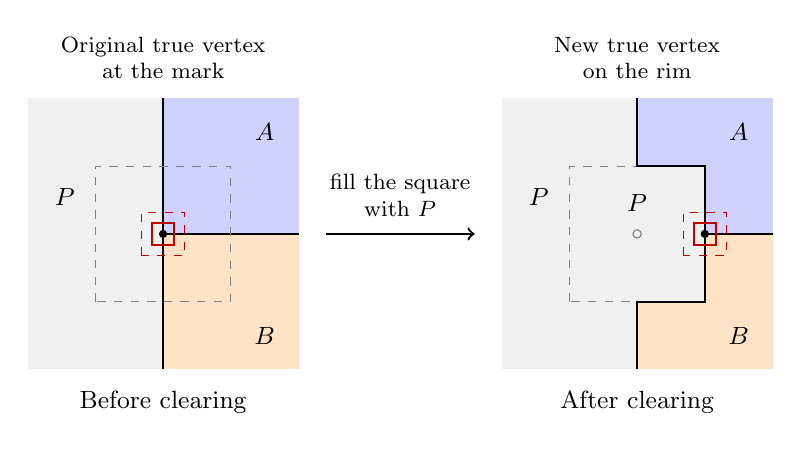
\begin{tikzpicture}[x=0.86cm,y=0.86cm,font=\small]
  \begin{scope}[shift={(-3.5,0)}]
    \fill[gray!12] (-2,-2) rectangle (2,2);
    \fill[blue!18] (0,0) rectangle (2,2);
    \fill[orange!22] (0,-2) rectangle (2,0);
    \draw[thick] (0,-2)--(0,2);
    \draw[thick] (0,0)--(2,0);
    \draw[dashed,gray] (-1,-1) rectangle (1,1);
    \draw[red!75!black,thick] (-0.16,-0.16) rectangle (0.16,0.16);
    \draw[red!75!black,dashed] (-0.32,-0.32) rectangle (0.32,0.32);
    \fill (0,0) circle (1.5pt);
    \node at (-1.45,0.55) {$P$};
    \node at (1.5,1.5) {$A$};
    \node at (1.5,-1.5) {$B$};
    \node[below] at (0,-2.18) {Before clearing};
    \node[above,align=center,font=\footnotesize] at (0,2.15)
      {Original true vertex\\at the mark};
  \end{scope}
  \draw[->,thick] (-1.1,0)--(1.1,0);
  \node[above,align=center,font=\footnotesize] at (0,0.12)
    {fill the square\\with $P$};
  \begin{scope}[shift={(3.5,0)}]
    \fill[gray!12] (-2,-2) rectangle (2,2);
    \fill[blue!18] (0,0) rectangle (2,2);
    \fill[orange!22] (0,-2) rectangle (2,0);
    \fill[gray!12] (-1,-1) rectangle (1,1);
    \draw[dashed,gray] (-1,-1) rectangle (1,1);
    \draw[thick] (0,2)--(0,1)--(1,1)--(1,-1)--(0,-1)--(0,-2);
    \draw[thick] (1,0)--(2,0);
    \draw[red!75!black,thick] (0.84,-0.16) rectangle (1.16,0.16);
    \draw[red!75!black,dashed] (0.68,-0.32) rectangle (1.32,0.32);
    \fill (1,0) circle (1.5pt);
    \draw[gray] (0,0) circle (1.5pt);
    \node at (-1.45,0.55) {$P$};
    \node at (0,0.45) {$P$};
    \node at (1.5,1.5) {$A$};
    \node at (1.5,-1.5) {$B$};
    \node[below] at (0,-2.18) {After clearing};
    \node[above,align=center,font=\footnotesize] at (0,2.15)
      {New true vertex\\on the rim};
  \end{scope}
\end{tikzpicture}
\caption{A point treatment for three distinct labels, shown in units of
$t$.  The dashed gray square is the radius-one treated square; solid
black lines are actual label interfaces.  After filling with $P$, the
only true vertex in this example is the meeting of $P,A,B$ on the right
rim.  The other ray/rim contacts involve only two labels.  Red solid
and dashed squares illustrate the inner and outer holes at the actual
true vertices, enlarged for visibility.  In the protocol their radii are
$h_n$ and $2h_n$, with one uniformly small $\epsilon_0$; the same
construction handles the finitely many ray patterns in the proof.}
\label{fig:geometry-points}
\end{figure}


For a birth or death, a point of the remaining closed changed region
lies outside the interiors of the treated squares.  Consequently
$d_{\mathcal V}(y)\ge t$, and homogenization to the surrounding label
can only remove its other-label obstructions.  By
\eqref{eq:geometry-birth-clearance}, after decreasing a fixed constant
if necessary, its separation from the other labels is bounded below by
\begin{equation}
 a_1\max\{t,\min(n,d_{\mathcal V}(y))\},
 \qquad a_1>0.
 \label{eq:geometry-floor}
\end{equation}
Every true vertex of the surrounding temporary guide belongs to the
closure of positions of labels different from $P_\circ$.  Enlarging
such a center to its outer hole square subtracts at most $2h_n$ from
this separation.  Since $h_n=\epsilon_0t$ in the present large-scale
case, a further fixed decrease of $a_1$ preserves
\eqref{eq:geometry-floor} for all outer hole sites too.

There are no changed true vertices in the bulk recoloring.  To see
this also at the treated rims, the closure of the truncated changed
region has a positive neighborhood containing only $P_\circ$ in the
surrounding guide.  A birth or reversed death introduces only one
additional label in that neighborhood.  Thus any newly drawn
interface, including where it meets a treated-square rim, has at most
two incident labels.  Existing true vertices are separated from this
closed change and retain their guides, holes, and tag holders.  The
raw target $T$ is therefore outside all holes, compactly located in
diameter $O(n)$, and satisfies the tapering hypothesis against the set
$E$ consisting of other owners and all outer hole sites.  The remaining
raw buffer has a single owner.  Lemma~\ref{lem:birth}, in its forward
or reverse form, implements the bulk change.

For the exchange, homogenization removes all noncommon-$C$ positions
inside the treated squares.  By
\eqref{eq:geometry-exchange-clearance}, every remaining such position
has the same floor at $t$ in its distance from $\partial Y$.  This
also holds for new rim vertices: a rim true vertex belongs to the
closure of an outside sector that is not $C$, and the original angular
estimate applies at that point.  Thus $\partial Y$, including each of
its intersections with a treated-square rim, lies in an open
common-$C$ corridor.  No new true vertex is created by exchanging
the guides along that boundary.

Every true vertex on either sheet belongs to the closure of a
noncommon-$C$ region.  Its distance from $\partial Y$ is at least a
fixed multiple of $t$ in a treated neighborhood, and obeys the larger
angular bound elsewhere.  The full outer hole square, of radius
$2\epsilon_0t$, therefore lies strictly on one side of the lens
boundary.  The same tapered bound holds at every point of an outer hole, not only
at its center: both $y\mapsto\dist(y,\partial Y)$ and
$y\mapsto d_{\mathcal V}(y)$ are $1$-Lipschitz. If $c$ is the center
and $|x-c|_\infty\le2\epsilon_0t$, put
$Q_x=\max\{t,\min(n,d_{\mathcal V}(x))\}$. A center clearance
$a_*\max\{t,\min(n,d_{\mathcal V}(c))\}$ gives
\[
 \dist(x,\partial Y)\ge a_*Q_x-2\epsilon_0(a_*+1)t
                   \ge \tfrac12a_*Q_x
\]
after fixing $\epsilon_0$ small enough. In particular, \emph{every}
selected variable-radius square in that hole lies on the same side,
since its radius is at most $2h_n$.  Exchanging a neighborhood of such a vertex substitutes one
complete sheet guide and carries its entire hole and tag.  It does
not splice sectors of two guides at a vertex.

For Lemma~\ref{lem:exchange}, let $T$ be the positions inside $Y$
that are not common $C$, together with all inside outer hole sites,
and let $E$ be the analogous set outside $Y$.  The set $T$ has
diameter $O(n)$.  Any segment from a point of $T$ to a point of $E$
crosses $\partial Y$, so its length is at least the distance of that
point of $T$ from the boundary.  The preceding clearance bounds,
including the outer-hole enlargement, therefore give the required
tapering separation of $T$ from $E$.  On the remaining positions both
raw copies are held by $C$.  This proves all hypotheses of the exchange
lemma, including its condition on whole holes and their tags.

All statements use actual labels.  Coalescing nominal labels cannot
create a meeting of three actual owners: the closure of an identified
region is the union of its finitely many former closures.  If a nominal
vertex disappears under such an identification, at most two actual
owners meet there and no vertex encoding is required.  The same
argument covers the exterior placeholder.  Empty physical targets
need no information estimate.

Choose one fixed $a>0$ smaller than all the surviving constants in
these tapering bounds.  Proposition~\ref{prop:angular}, at accuracy
$L^{-60}$, then supplies a sufficiently large fixed $D$ in
\eqref{eq:geometry-scales}.  The birth and exchange errors are
$O(L^{-30})$, as required by their lemmas.  The constants used to
choose $a$ depend only on the fixed geometric templates, not on $D$.

\subsection{The small-patch covers}

We verify every invocation of Lemma~\ref{lem:small-rewrite}.  The
following compactness observation makes the two-owner condition
uniform, including along the boundary of an inner hole.

Fix a compact working neighborhood and one scaled guide.  For each
actual label $c$, let $F_c$ be the closure of its region in that
neighborhood, with all open inner hole squares removed.  Each $F_c$
is compact.  No three $F_c$ with distinct actual labels have a common
point, because every true vertex lies strictly inside its own inner
hole.  It follows that there is a positive footprint diameter such
that no smaller footprint meets three of these sets.  Otherwise take
a sequence of shrinking footprints, pass to constant label choices
and convergent points in the compact working neighborhood, and obtain
a point common to three distinct $F_c$.

This remains uniform for our small-scale and resizing radius
parameters.  After scaling, these parameters range over compact
intervals bounded away from zero.  The joint sets of a parameter and
a point belonging to $F_c$ are closed: being outside an open square
is a non-strict distance inequality.  The same convergent-subsequence
argument applies to the joint sets.  There are only finitely many
label-equality types, so take the minimum positive footprint bound
over those types.  Apply the test separately to the old and new
guides, then take the smaller bound.  Different old and new hole
centers do not mix the two tests.

Notice that the \emph{center} of a footprint may lie inside a hole.
The condition counts labels only at footprint points outside the
relevant inner holes.  Thus this observation permits a net of small
patches to cover the \emph{whole outer} hole footprints, as required
by Lemma~\ref{lem:small-rewrite}.

\paragraph{Point homogenization and removal.}
For one mark in the large-scale case, work in its radius-$2t$
neighborhood.  Include as affected every old and new hole at the
marked center or on the treated-square rim.  These are all possible
changed true vertices, and their outer squares lie strictly inside
that neighborhood for small $\epsilon_0$.  There are no other holes
nearby.  In units of $t$, the old and new guides are from a finite
family of ray patterns, with or without the square clearing, and the
inner hole radius is $\epsilon_0$.

Choose a fixed sufficiently small $\nu>0$.  Patches with inner radius
$u=\nu t$, centered on a square net of mesh at most $u$, cover the
treated square and all affected outer holes.  Take the centers within
$u$ of the set to be covered.  With $\nu$ small, their outer squares
are still inside the working neighborhood and avoid every untouched
hole.  The compactness observation gives at most two old owners
outside the old inner holes and at most two new owners outside the
new inner holes in each outer patch.  The number of patches is fixed:
the working diameter is $O(t)$ and the patch radius is $\nu t$.
Their raw owners and affected tag holders are among the bounded list
of parties in this local diagram.  Apply
Lemma~\ref{lem:small-rewrite}, one mark and one sheet at a time.
The separated marked neighborhoods do not change one another's
diagrams.  The same verification applies when removing the point
treatment after the bulk operation, using its actual target guide.

\paragraph{Direct repainting when $n\le K_0t$.}
Before and after a direct repainting, true vertices are grid corners.
Only the four corners of the square being repainted can change their
true-vertex status or their tag holder.  Treat every old or new hole
at those corners as affected.  The hole radius obeys
\begin{equation}
 \frac{\epsilon_0}{\max(K_0,1)}
 \le \frac{h_n}{n}\le\epsilon_0.
 \label{eq:geometry-small-radius}
\end{equation}
In units of $n$, the old/new label patterns form a finite collection,
and the possible radius ratios lie in the displayed compact positive
interval.  The compactness observation gives a uniform sufficiently
small patch radius $u=\nu n$.  A fine net covers $S$ and the entire
affected outer holes with a fixed number of such patches.  Every
untouched grid-corner hole is a fixed scaled distance from the set to
be covered: corners of $S$ have all been included, and any other grid
corner is at distance at least $n$ from $S$.  Choosing $\epsilon_0$
and then $\nu$ small makes all outer patches avoid those holes.  All
hypotheses of Lemma~\ref{lem:small-rewrite} follow.  This
directly repaints $S$ without using an auxiliary sheet.

\paragraph{Hole resizing.}
Entering level $n$, the old and new radii are
$\epsilon_0\min(2n,t)$ and $\epsilon_0\min(n,t)$.  If they differ,
then $n<t$, in particular $n\le K_0t$, and their ratio lies between
one and two.  The current guide is unchanged and is uniform on
$2n$-blocks.  Resize one true-vertex hole at a time.  The union of
its two outer footprints has diameter $O(n)$; other true vertices
are separated on that scale.  The same compactness and fine-net
argument covers both footprints, avoids all other holes, and gives
the separate old/new two-owner tests.  Intermediate configurations
with some holes already resized obey the same positive radius and
separation bounds.  This proves the required small-patch rewrite for
each resize.

For completeness, these covers apply uniformly to every selected
adaptive radius in a rewrite branch.  A selected patch square
contains its inner square, so every changed raw site and every site
of an affected selected hole is intercepted by a patch.  A raw
input-to-output identity wire that remains unintercepted cannot
change owner.  An old-hole decoded ket therefore has no open leg
directly at a new raw output, and a new-hole encoding bra has none
directly at an old raw input.  Overlapping patches merely connect an
earlier patch ket to a later patch bra.  Open patch-bra legs come
from raw inputs outside all old inner holes, and open patch-ket legs
go to raw outputs outside all new inner holes.  Their owner counts
are exactly the separate two-owner counts just proved.  Thus the
geometric hypotheses give the branchwise support facts used in the
tensor expansion of Lemma~\ref{lem:small-rewrite}, even when old
and new holes have different radii.

There is no circular choice of constants.  First fix the band
templates and obtain $a_0$ and their radial-chart constants; then
choose $K_0$, then $\epsilon_0$, and then the fixed mesh parameter
$\nu$ from the compact families just described.  Choose the smaller
clearance $a$ and the information scale constant $D$ afterward.
Finally choose $B_0$ large enough that all hole radii and all added
patch radii are at most $B_0\log L$.  A fixed multiple of $K_0D$
suffices, since the point patches have size $O(t)$, the direct
patches have size $O(n)\le O(K_0t)$, and all holes have size $O(t)$.
The adaptive patch ranks may depend on this fixed $B_0$, but every
selected support still lies between its predetermined inner and
outer square, so no geometric constant has to be chosen again.

\subsection{Party lifetimes and the protocol bounds}

Each elementary birth, death, or exchange has a fixed number of
marks.  The point treatments have a fixed number of patches and
parties.  The edge word uses a fixed number of elementary operations
and four auxiliary sheets at most per repainting.  Consequently each
repainting, and each junction resize, uses a uniformly bounded
number of linked gates and parties.  Small-patch rewrites can be
replaced by arbitrarily accurate polynomial expansions and rescaled
near one to remain contractions.  Together with the $L^{-60}$ patch
tests and the $O(L^{-30})$ splitting errors, choose their precision
so that each change has reference-vector error at most $C L^{-20}$.

At a level-$n$ repainting, every active main owner is an $n$- or
$2n$-block owner.  On the affected footprints those blocks lie at
distance $O(n)$ from the repainted square.  The same is true of
their tag holders, since tags are held by incident labels.  An
auxiliary uses only the labels of the local edge and point diagrams;
its uniform initial owner $C$ is the actual neighboring-block owner,
even though it privately holds a whole copy of $\Omega$.  The
placeholder party is attached to the repainted block at scale $n$.
Resizing uses the current block labels near its junction.  Private
buffer isometries may act on registers at much more distant physical
positions, but create no additional party or link.

The following stronger invariant concerns active main owners; the
inactive exterior placeholder is omitted at the start and end of a
level. It proves the lifetime claim, rather than just locality at an
individual step:
\begin{equation}
 \begin{aligned}
  \text{start of level }n &: \text{ only }2n\text{-block main labels};\\
  \text{during level }n &: \text{ only }2n\text{- and }n\text{-block main labels,
       plus its temporary placeholder};\\
  \text{end of level }n &: \text{ only }n\text{-block main labels}.
 \end{aligned}
 \label{eq:geometry-active-labels}
\end{equation}
Main tags always use incident non-placeholder labels.  Hence a party
of side $m$ disappears from every main tag as well as every main
guide region by the end of level $m/2$.  In particular, when the last
incident child square repaints, its corner rewrite updates the tag
at that junction.  Resizing introduces no obsolete owner.  Thus
this party can occur in linked gates only at levels $m$ and $m/2$
and their intervening transition.  At these scales there are only
a fixed number of repaintings or junctions within distance $O(m)$
of its block.

Frozen auxiliary frames do not invalidate this invariant.  Each is
initialized, used in its one edge construction, returned from its
point treatment to its specified final frame, and permanently
retired before the repainting ends.  Its remaining entangled
registers and tags are kept idle at their owners.  No subsequent
gate undoes that exchange, and no later auxiliary initialization
consults a frozen label: its $C$ is always selected from the current
main guide.  Therefore frozen memory contributes no further linked
incidence.  The same applies to a retired placeholder party.  A
fresh placeholder identity at the next repainting has no raw main
register or persistent main tag to inherit.  This proves a uniform
bound on every party's total linked participation.

For later routing, a square of side $n=2^j$ and block indices $(r,s)$
has the integer address
\begin{equation}
 a(S)=
 \begin{cases}
 (nr+n/2,\,ns+n/2),&j\ge1,\\
 (r,s),&j=0.
 \end{cases}
 \label{eq:geometry-addresses}
\end{equation}
Use the same address for its additional parties.  The preceding
locality statement gives $O(n)$ address distances for parties sharing
a gate, and their scales are equal or adjacent.  The addresses lie
in $\{0,\ldots,N-1\}^2$; unit-square physical outputs have their
actual site indices as addresses.

There are $O((N/n)^2)$ repaintings and junctions at scale $n$.
Summing over dyadic scales gives $O(N^2)=O(L^2)$ in total.  The number
of block parties, additional parties, auxiliary sheets, and changes
is therefore $O(L^2)$, and in particular bounded by $C L^3$.
Each frozen auxiliary has only a fixed number of holes: its guide
differs from its uniform guide only in one bounded edge template and
its endpoint treatments.  Even the weaker total bound $C L^3$ on
frozen auxiliary holes will suffice.

Initialize all required copies of $\Omega$ privately at their future
owners, including the main copy at the root.  This is a pure product
initialization across parties, with no restriction on private state
complexity.  At the beginning the main guide has only the root label
and the exterior placeholder, so it has no true vertex and no hole.
At every stage use the tensor product of the designated main frame,
active auxiliary frames, idle initial copies, and frozen final
auxiliary frames as its reference vector.  Untouched factors have
norm at most one, so the local reference-error bounds remain valid
with all these spectators.

At level $n=1$, choose $\epsilon_0<1/4$.  A grid-corner outer hole
then has radius $2\epsilon_0<1/2$ and contains no cell-center physical
site.  Its encoding is trivial.  Thus all remaining main registers
are raw at their unit-square parties and the main reference is
exactly $\Omega$, apart from trivial tags.  The other reference
factors comprise $\Xi$.  Each encoded auxiliary frame has norm at
least one minus its number of holes times $L^{-60}$, by the frame
constraint and contraction bounds.  Multiplying these lower bounds
and using the total frozen-hole count gives
$1-C L^{3-60}\le\norm{\Xi}\le1$.  All auxiliary registers and all
nonphysical outputs can be discarded party by party.

This proves every assertion of Proposition~\ref{prop:protocol}.
